\chapter{Modelling and Simulation}

\graphicspath{{./Figures/Modelling and Simulation}}

In this pivotal chapter, we meticulously derive the center of gravity and the moment of inertia for the two-wheeled self-balancing robot.
These parameters are the linchpins of our dynamic analysis, serving as the critical variables within the equations of motion that govern the robot's behavior.
By calculating these values with precision, we can substitute them into our dynamic equations, thereby tailoring the model to reflect the true dynamics of the robot.
This process not only enhances the accuracy of our simulations but also ensures that the control strategies developed are based on a robust and representative model of the robot's physical capabilities.
The careful derivation of these parameters is a testament to the thoroughness of our approach, ensuring that the resulting model is both reliable and predictive of the robot's real-world performance.
\newpage

\section{Mathematical Modelling}

%	\item \textbf{TWIPR Model:} Explanation of the Two-Wheeled Inverted Pendulum Robot (TWIPR) model.
The two-wheeled Inverted Pendulum robot model is as shown in the figure where it consists of two legs that include a hip and knee joints as well as wheels at the end of each leg.
The robot needs to constantly adjust its posture to be able to maintain the balance, just like how the human being balances when standing on the feet.
This new TWIPR model is the latest iteration in the evolution of its predecessor.

%Two subfigures side by side of the two models 	the old model and the new model
\begin{figure}[h]
	\centering
	\begin{subfigure}[t]{0.45\textwidth}
		\centering
		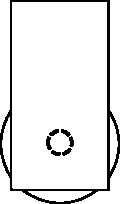
\includegraphics[height=0.7\textwidth]{Old model}
		\caption{Old model}
		\label{fig:Old model}
	\end{subfigure}
	\begin{subfigure}[t]{0.45\textwidth}
		\centering
		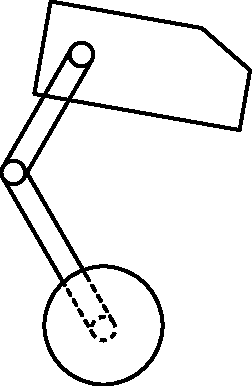
\includegraphics[height=0.7\textwidth]{New model}
		\caption{New model}
		\label{fig:New model}
	\end{subfigure}
	\caption{Comparison between the old and new models}
	\label{fig:Comparison between the old and new models}
\end{figure}

%	\item \textbf{Focus on 2D Dynamics:} Discussion on the scope limited to 2D dynamics and plans for future expansion to 3D dynamics and controller synthesis.
\subsection{2D Dynamics}
The scope of this project is limited to 2D dynamics.
However, the model can be extended to 3D dynamics and controller synthesis for the 3D dynamics in the future.
The 2D dynamics is considered for simplification purposes and to reduce the complexity of the model.
The 2D dynamics modeling takes into account the robot's movement in the x-y plane and the rotation of the knee joint, hip joint, and the wheels around the z-axis.
The 2D dynamics modeling considers one leg and half of the body mass.
%	\item \textbf{Assumptions and Parameters:} Detailing assumptions such as considering motor angles as parameters.
	%the cansilation of the radial forces and the assumption of the motor angles as parameters.
\subsection{Assumptions and Parameters}
Many assumptions were made to simplify the model and reduce the complexity of the calculations.The weights and the lengths of the links are constant, and the angles $\phi_2$, $\phi_3$ are input variables that can be controlled to adjust the robot's posture.
%table of the assumptions
	\begin{table}[h!]
		\centering
		\caption{Parameters of the mechanical system}
		\label{tab:parameters}
		\begin{tabular}{lcl}
			\toprule
			Parameter & Value & Description \\
			\midrule
			$L_1$ & 0.017 m & Length of the Wheel knee Link \\
			$L_2$ & 0.017 m & Length of the Body knee Link \\
			$L_{C1}$ & 0.013 m & Distance between the Wheel Joint and the center of mass of the Wheel knee Link \\
			$L_{C2}$ & 0.013 m & Distance between the Knee Joint and the center of mass of the Body knee Link \\
			$L_{C3}$ & 0.013 m & Distance between the Hip Joint and the center of mass of the body \\
			$m_{L1}$ & 0.1 kg & Mass of the Wheel knee Link \\
			$m_{L2}$ & 0.1 kg & Mass of the Body knee Link \\
			$m_K$ & 0.1 kg & Mass of the Knee Joint \\
			$m_B$ & 0.1 kg & Mass of the Body \\
			$L_G$ & - & Distance between the center of gravity and the Wheel Joint \\
			$\theta$ & - & Angle between the center of gravity and the Wheel knee Link \\
			$\phi_1$ & - & Angle between the Body knee Link and the $y_B$ vertical axis of the body \\
			$\phi_2$ & - & Angle between the Wheel knee Link and the Body knee Link \\
			$\phi_3$ & - & Angle between the Body knee Link and the center of mass of the body \\
			$\phi_4$ & - & Angle between the Body knee Link and the $X_B$ horizontal axis of the body \\
			\bottomrule
		\end{tabular}
	\end{table}


%	\item \textbf{Model Derivation for \textit{l\_cg} and \textit{I\_y}:} Derivation of the models for center of gravity length (\textit{l\_cg}) and inertia around the y-axis (\textit{I\_y}).
%Center of Gravity
\newpage
\subsection{Center of Gravity }
%	$\bullet$ in that section the calculations of the overall center of gravity
%
%	$\bullet$ Significance in Dynamics:The stability of an object is directly impacted by the COG position, which also affects how it reacts to forces and moments from the outside world.
%
%	$\bullet$ Maintain equilibrium,
%
%	$\bullet$ accurately determining the COG is crucial for predicting and controlling dynamic behavior
%
%	in the above figure in order to simplify the deriviation of the center of

The calculation of the center of gravity is crucial for the dynamic analysis of the robot.
The center of gravity is calculated by taking into account the weights of the links, the knee joint, the body and the distances between these weights and the local coordinate system of the robot.
The stability of the robot is directly impacted by the center of gravity position, which also affects how it reacts to forces and moments from the outside world.
The following equations are used to calculate the center of gravity location referencing the local coordinate system of the robot.
% input the model figure from the graphics path
	\begin{figure}[h]
		\centering
		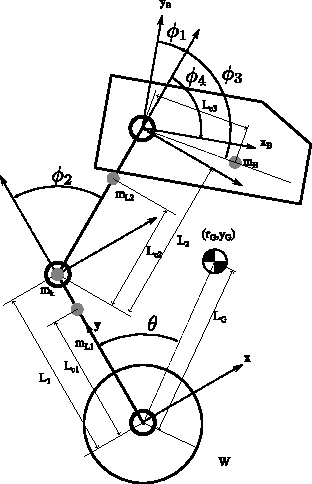
\includegraphics[width=.5\textwidth]{Model}
		\caption[Mechanical model with the local coordinate system]{Figure illustrating the mechanical model with the local coordinate system to determine the center of gravity.}
		\label{Mechanical model with the local coordinate system}
	\end{figure}

	\begin{equation}
		\begin{aligned}
			x_{CG} = \frac{m_{L1} \cdot 0 + m_K \cdot 0 + m_{L2} \cdot L_{C2} \cdot \sin(\phi_2) + m_B \cdot (L_2 \cdot \sin(\phi_2) + L_{C3} \cdot \sin(\phi_2 + \phi_3))}{m_{L1} + m_{L2} + m_K + m_B}
		\end{aligned}
	\end{equation}

	\begin{equation}
		\begin{aligned}
			y_{CG} = \frac{m_{L1} \cdot L_{C1} + m_K \cdot L_1 + m_{L2} \cdot (L_1 + L_{C2} \cdot \cos(\phi_2)) + m_B \cdot (L_1 + L_2 \cdot \cos(\phi_2) + L_{C3} \cdot \cos(\phi_2 + \phi_3))}{m_{L1} + m_{L2} + m_K + m_B}
		\end{aligned}
	\end{equation}

%expain the equations in more details
	\begin{equation}
		L_G = \sqrt{x_{CG}^2 + y_{CG}^2}
	\end{equation}

	\begin{equation}
		\theta = \arctan\left(\frac{{x_{CG}}}{{y_{CG}}}\right)
	\end{equation}

	\begin{figure}[h]
		\centering
		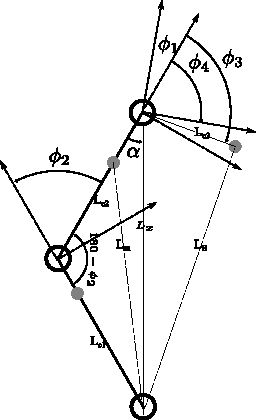
\includegraphics[width=.5\textwidth]{Angles}
		\caption[Moment of inertia Schematic representation]{Schematic representation detailing the requisite angles and lengths for calculating the moment of inertia.}
		\label{fig:Schematic representation xxxxx detailing the requisite angles and lengths for calculating the moment of inertia.}
	\end{figure}

	\subsection{Moment of inertia}
	%MOI
	Moment of inertia calculations
	\begin{equation}
		L_m = \sqrt{L_1^2 + L_{C2}^2 - L_1 L_{C2} \cos(180 - \phi_2)}
	\end{equation}

	\begin{equation}
		L_{x} = \sqrt{L_1^2 + L_2^2 - L_1 L_2 \cos(180 - \phi_2)}
	\end{equation}


	\begin{equation}
		\alpha = \cos^{-1} \left( \frac{l_2^2 + l_{x}^2 - l_1^2}{2 l_2 l_{x}} \right)
	\end{equation}

	%explain the equations in more details

	\begin{equation}
		L_b = \sqrt{L_{x}^2 + L_{C3}^2 - Lx L_{C3} \cos(180 - \alpha - \phi_3 )}
	\end{equation}

	\begin{equation}
		I_{L1} = \frac{1}{12} m_{L1} (a_1^2 + b_1^2)
	\end{equation}
	\begin{equation}
		I_{L2} = \frac{1}{12} m_{L1} (a_2^2 + b_2^2)
	\end{equation}
	\begin{equation}
		I_K = \frac{1}{2} m_K R_m^2
	\end{equation}
	\begin{equation}
		I_B = \frac{1}{12} m_B (a_B^2 + b_B^2)
	\end{equation}
	\begin{equation}
		I = I_{L1} + m_{L1} L_{C1}^2 + I_K + m_K L_1^2 + I_{L2} + m_{L2} L_m^2 + I_B + m_B L_b^2
	\end{equation}
%	\item \textbf{Integration into TWIPR Model:} Integration of derived models into a new TWIPR framework.

%	\item \textbf{Linear Model Derivation:} Derivation of the linear model from the integrated TWIPR model.

%	\item Modeling allows for predictive analysis and understanding of the robot's behavior.
	In order to predict the behavior of the robot under different settings, the modeling procedure entails constructing mathematical representations of the robot's dynamics and control systems.
%\end{itemize}






	\subsection{Equation of motion }
	%equation of motion 
	Equation of motion 
	
	
		\subsection{Dynamics of the Two-Wheeled Inverted Pendulum Robot}
	Given the functions $B_i: \mathbb{R} \rightarrow \mathbb{R}$, $C_{ij}: \mathbb{R} \rightarrow \mathbb{R}$, $D_{ij}: \mathbb{R} \rightarrow \mathbb{R}$, and $V_i: \mathbb{R} \rightarrow \mathbb{R}$, $i,j \in \{1,2,3\}$, the equations of motion are given by:

	\begin{align}
		\ddot{s} &= \frac{\sin(\Theta)}{V_1(\Theta)} \left( -C_{11}(\Theta)g + C_{12}\dot{\Theta}^2 + C_{13}(\Theta)\dot{\psi}^2 \right) - \frac{D_{11}(\Theta)}{V_1(\Theta)}\dot{s} + \frac{D_{12}(\Theta)}{V_1(\Theta)}\dot{\Theta} + \frac{B_{1}(\Theta)}{V_1(\Theta)}(\tau_L + \tau_R) \\
		\ddot{\Theta} &= \frac{\sin(\Theta)}{V_1(\Theta)} \left( C_{21} - C_{22}(\Theta)\dot{\Theta}^2 - C_{23}(\Theta)\dot{\psi}^2 \right) + \frac{D_{21}(\Theta)}{V_1(\Theta)}\dot{s} - \frac{D_{22}(\Theta)}{V_1(\Theta)}\dot{\Theta} - \frac{B_{2}(\Theta)}{V_1(\Theta)}(\tau_L + \tau_R)  \\
		\ddot{\psi} &= \frac{\sin(\Theta)}{V_2(\Theta)} \left( C_{31}(\Theta)\dot{\Theta}\dot{\psi} - C_{32}(\Theta)\dot{\psi}\dot{s} \right) - \frac{D_{33}(\Theta)}{V_2(\Theta)}\dot{\psi} - \frac{B_{3}}{V_2(\Theta)}(\tau_L - \tau_R)
	\end{align}


	The equations of motion are derived in [44]. The functions $B_i: \mathbb{R} \rightarrow \mathbb{R}$, $C_{ij}: \mathbb{R} \rightarrow \mathbb{R}$, $D_{ij}: \mathbb{R} \rightarrow \mathbb{R}$, and $V_i: \mathbb{R} \rightarrow \mathbb{R}$, $i,j \in \{1,2,3\}$, are given by:

	\begin{equation}
		C_{11}(\Theta) = m_B^2 l^2 \cos(\Theta)g,
	\end{equation}
	\begin{equation}
		C_{12} = (I_2 + m_B l^2) m_B l,
	\end{equation}
	\begin{equation}
		C_{13}(\Theta) = (I_2 + m_B l^2) m_B l + m_B l (I_3 - I_1 - m_B l^2) \cos^2(\Theta),
	\end{equation}
	\begin{equation}
		C_{21} = (m_B + 2m_W + \frac{2J}{r^2}) m_B l,
	\end{equation}
	\begin{equation}
		C_{22}(\Theta) = m_B^2 l^2 \cos(\Theta),
	\end{equation}
	\begin{equation}
		C_{23}(\Theta) = m_B^2 l^2 + (m_B + 2m_W + \frac{2J}{r^2}) (I_3 - I_1 - m_B l^2) \cos(\Theta).
	\end{equation}
	\begin{equation}
		C_{31}(\Theta) = 2 (I_3 - I_1 - m_B^2) \cos(\Theta),
	\end{equation}
	\begin{equation}
		C_{31} = m_B l,
	\end{equation}
	\begin{equation}
		D_{11}(\Theta) = \frac{(I_2 + m_B^2) 2c_\alpha}{r^2} - \frac{m_B \cos(\Theta) 2c_\alpha}{r},
	\end{equation}
	\begin{equation}
		D_{12}(\Theta) = \frac{(I_2 + m_B^2) 2c_\alpha}{r} - 2m_B \cos(\Theta) c_\alpha,
	\end{equation}
	\begin{equation}
		D_{21}(\Theta) = \frac{(m_B + 2m_W + \frac{2J}{r^2}) 2c_\alpha}{r} + \frac{m_B \cos(\Theta) 2c_\alpha}{r^2},
	\end{equation}
	\begin{equation}
		D_{22}(\Theta) = \frac{(m_B + 2m_W + \frac{2J}{r}) 2c_\alpha + m_B \cos(\Theta) 2c_\alpha}{r},
	\end{equation}
	\begin{equation}
		D_{33}(\Theta) = \frac{d^2}{2r^2 c_\alpha},
	\end{equation}
	\begin{equation}
		B_{1} = \frac{(I_2 + m_B^2) \frac{1}{r} + m_B \cos(\Theta)}{r},
	\end{equation}
	\begin{equation}
		B_{2} = \frac{m_B l}{r} - \cos(\Theta) + m_B + 2m_W + \frac{2J}{r^2},
	\end{equation}
	\begin{equation}
		B_{3} = \frac{d}{2r},
	\end{equation}
	\begin{equation}
		V_{1} = (m_B + 2m_W + \frac{2J}{r^2}) (I_2 + m_B^2) - m_B^2 \cos^2(\Theta),
	\end{equation}
	\begin{equation}
		V_{2} = I_3 + 2K + (m_W + \frac{J}{r^2}) \frac{d^2}{2} - (I_3 - I_1 - m_B^2) \sin^2(\Theta).
	\end{equation}


	\begin{table}[h!]
		\centering
		\caption{Parameters of the mechanical system}
		\label{tab:parameters}
		\begin{tabular}{lcl}
			\toprule
			Parameter & Value & Description \\
			\midrule
			$m_B$ & 2.5 kg & mass of the pendulum body \\
			$m_W$ & 0.636 kg & mass of a wheel \\
			$l$ & 0.026 m & distance between the wheel axis and the pendulum's center of gravity \\
			$d$ & - & distance between the two wheels \\
			$J$ & \(5.175 e^{-4}\) kgm\textsuperscript{2} & moment of inertia of a wheel w.r.t. Reference frame \{C\} in direction of \(c_2\) \\
			$K$ & - & moment of inertia of a wheel w.r.t. reference frame \{C\} in direction of \(c_3\) \\
			$I_1$ & - & moment of inertia of pendulum's body w.r.t. Reference frame \{B\} in direction of \(b_1\) \\
			$I_2$ & \(0.0165\) kgm\textsuperscript{2} & moment of inertia of pendulum's body w.r.t. Reference frame \{B\} in direction of \(b_2\) \\
			$I_3$ & - & moment of inertia of pendulum's body w.r.t. Reference frame \{B\} in direction of \(b_3\) \\
			$c_\alpha$ & \(4.630 e^{-4}\) Nms & viscous friction coefficient \\
			\bottomrule
		\end{tabular}
	\end{table}
	
	
	



\section{Numerical Simulation}
\begin{itemize}
	\item \textbf{Discrete Numerical Simulation:} Elaboration on the process of discrete numerical simulation, including the discrete double integration method to arrive at the state vector.
\end{itemize}

\section{Simulation Environment}
%figure of the simulation environment
\subsection{Overview of the Simulation Environment}
\subsection{spaces}

%\begin{itemize}
%	\item \textbf{Overview of the Simulation Environment:} A brief overview of the simulation environment, referencing David's Bachelor Thesis for details.
%
%
%	\item \textbf{Integration of the Model:} Description of integrating the new TWIPR model into the simulation environment and a summary of the individual components of the model.
%\end{itemize}

\section{Controller Synthesis}
%\begin{itemize}
%	\item \textbf{State-Space Controllers:} Introduction to two state-space controllers: Linear Quadratic Regulator (LQR) and Pole-Placement.

%figure of the state space controller
\begin{figure}[h]
	\centering
	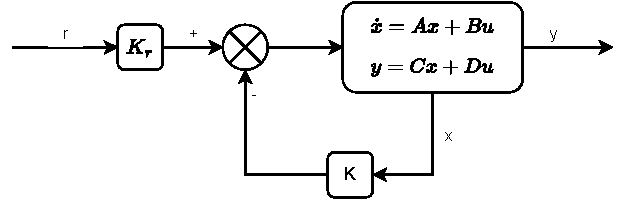
\includegraphics[width=.5\textwidth]{Block Diagram of State Feedback Controller}
	\caption{Block diagram of a state feedback controller}
	\label{fig:Block diagram of a state feedback controller}
\end{figure}


In the realm of modern control theory, State-Space controllers are a pivotal component for managing the behavior of complex systems.Among the most prominent of these controllers are the Linear Quadratic Regulator (LQR) and Pole-Placement controllers, both of which are robust and effective in various applications.
This section provides an overview of these controllers and their application to the legged TWIPR robot.
%full state feedback controllers

\subsection{Linear Quadratic Regulator (LQR)}
The Linear Quadratic Regulator (LQR) is a state-space controller that uses a quadratic cost function to determine the optimal control input for a given system. It aims to minimize the cost function by adjusting the control input, thereby ensuring that the system's state converges to the desired state. The LQR controller is defined by the following equation:
\begin{equation}
	u(t) = -Kx(t)
\end{equation}
where $u(t)$ is the control input, $x(t)$ is the state vector, and $K$ is the gain matrix. The gain matrix is calculated using the following equation:
\begin{equation}
	K = R^{-1}B^TP
\end{equation}
where $R$ is the control weight matrix, $B$ is the input matrix, and $P$ is the solution to the Riccati equation:
\begin{equation}
	A^TP + PA - PBR^{-1}B^TP + Q = 0
\end{equation}
where $A$ is the state matrix and $Q$ is the state weight matrix. The state matrix, state weight matrix, and control weight matrix are defined as follows:
%A = [ 0.5403, -0.8415; 0.8415,  0.5403];
%\begin{equation}
%	A = \begin{bmatrix}
%		0.5403 & -0.8415 \\
%		0.8415 & 0.5403
%	\end{bmatrix}
%\end{equation}
\begin{equation}
	Q = \begin{bmatrix}
		1 & 0 \\
		0 & 1

	\end{bmatrix}
\end{equation}
\begin{equation}
	R = \begin{bmatrix}
		1
	\end{bmatrix}
\end{equation}
The LQR controller is implemented in the simulation environment using the \textit{Python Control Systems Library} \cite{python_control2021}.

\subsection{Pole-Placement Technique}
The Pole-Placement technique is a state-space controller that uses the Ackermann formula to determine the optimal control input for a given system. It aims to place the poles of the system at the desired locations by adjusting the control input, thereby ensuring that the system's state converges to the desired state.placing the poles is not initiutive for high order systems or systems with multiple actuators. The Pole-Placement controller is defined by the following equation:
\begin{equation}
	u(t) = -Kx(t)
\end{equation}
where $u(t)$ is the control input, $x(t)$ is the state vector, and $K$ is the gain matrix. The gain matrix is calculated using the following equation:
\begin{equation}
	K = \begin{bmatrix}
		k_1 & k_2 & k_3
	\end{bmatrix}
\end{equation}
where $k_1$, $k_2$, and $k_3$ are the gains for the first, second, and third states, respectively. The gains are calculated using the following equation:
\begin{equation}
	k_i = \frac{1}{b_i} \left( \sum_{j=0}^{n-1} a_{n-j} \alpha_{i+j} - \alpha_i \right)
\end{equation}
where $a_i$ is the coefficient of the characteristic polynomial, $b_i$ is the coefficient of the denominator polynomial, and $\alpha_i$ is the desired location of the $i$th pole. The characteristic polynomial and denominator polynomial are defined as follows:
\begin{equation}
	a_i = \begin{cases}
		1 & i = 0 \\
		0 & i \neq 0
	\end{cases}
\end{equation}
\begin{equation}
	b_i = \begin{cases}
		1 & i = 0 \\
		0 & i \neq 0
	\end{cases}
\end{equation}
The Pole-Placement controller is implemented in the simulation environment using the \textit{Python Control Systems Library} \cite{python_control2021}.
%	\item \textbf{Configuration Specificity:} Explanation of how these controllers are specific to one configuration (knee angle and hip angle) of the robot.
\subsection{Configuration Specificity}
These controllers are specific to one configuration for the knee angle and hip angle of the robot.
Retuning the controllers is required when the configuration changes.
%	\item \textbf{Controller Retuning Algorithm:} Presentation of an algorithm for retuning the controllers as the configuration changes.
%\end{itemize}
\begin{lstlisting}[language=Python, caption=Changing the knee and hip angles of the robot, label={lst:Changing the knee and hip angles of the robot}]
    def change_knee_angle(self):
        self.agent1.set_leg_angles(hip_angle=self.agent1.dynamics.model.hip_angle,
                                   knee_angle=self.agent1.dynamics.model.knee_angle + deg2rad(5))

    def change_hip_angle(self):
        self.agent1.set_leg_angles(hip_angle=self.agent1.dynamics.model.hip_angle + deg2rad(5),
                                   knee_angle=self.agent1.dynamics.model.knee_angle)
\end{lstlisting}
where The code \ref{lst:Changing the knee and hip angles of the robot} Shows the functions that changes the knee and hip angles of the robot.
\begin{lstlisting}[language=Python, caption=Changing the knee and hip angles in the dynamics and retuning the controller, label={lst:Changing the knee and hip angles in the dynamics and retuning the controller}]
    def set_leg_angles(self, knee_angle: float, hip_angle: float):
        self.dynamics.model.knee_angle = knee_angle
        self.dynamics.model.hip_angle = hip_angle
        self.linear_dynamics = TWIPR_3D_Linear(self.dynamics.model, Ts, self.poles, self.eigenvectors)
        self.state_ctrl_K = np.hstack((np.zeros((2, 1)), self.linear_dynamics.K))
\end{lstlisting}
In the above code \ref{lst:Changing the knee and hip angles in the dynamics and retuning the controller} It hows the function that changes the knee and hip angles in the dynamics and retunes the controller.


\section{Simulation Analysis}
%\begin{itemize}
%	\item \textbf{Controller Responses:} Analysis of step response and responses to other inputs using one of the controllers in different configurations.
\subsection{Controller Responses}
In order to analyze the performance of the controllers, we conducted a series of simulations to evaluate their responses to various inputs.

%	\item \textbf{Impact of Non-Retuning:} Discussion on the effects of not retuning the controllers.
\subsection{Impact of Non-Retuning}

%	\item \textbf{Influence of Leg Configuration:} Analysis of how leg configuration influences the robot's behavior.
\subsection{Influence of Leg Configuration}
%	\item \textbf{Controller Setting Comparisons:} Comparative study of different controller settings and a comparison between LQR and Pole-Placement controllers.
\subsection{Controller Setting Comparisons}
%	\item \textbf{Optimal Controller Configuration:} Conclusion on which controller configuration might be best suited for such a robot.
%\end{itemize}
+










	


